\documentclass[12pt]{article}

\usepackage{amsmath}
\usepackage{amsthm}
\usepackage{amssymb}
\usepackage{mathrsfs}
\usepackage{setspace}
\usepackage{graphicx}
\usepackage{caption}
\usepackage{subcaption}
\usepackage{minted}

\newcommand{\w}{\omega}
\renewcommand{\a}{\alpha}
\renewcommand{\d}{\delta}
\newcommand{\s}{\sigma}
\newcommand{\e}{\epsilon}
\newcommand{\m}{\mu}
\newcommand{\p}{\rho}
\newcommand{\g}{\gamma}
\renewcommand{\b}{\beta}

\newcommand{\inn}[1]{\left\langle #1 \right\rangle}
\newcommand{\norm}[1]{\left\Vert #1 \right\Vert}
\newcommand{\abs}[1]{\left\vert #1 \right\vert}

\newcommand{\real}{\mathbb{R}}
\renewcommand{\int}{\mathbb{Z}}
\newcommand{\nat}{\mathbb{Z}^+}

\begin{document}

\title{Homework 8}
\date{\today}
\author{Hunter Schwartz}
\maketitle

%\doublespacing

\textbf{Problem 1}

(a) To satisfy the boundary conditions, we have $u(0,t) = \sin(0)e^{\b t} = 0$ for any given $\a$, but we also need $u(L,t) = \sin(\a L) e^{\b t} = 0$. Since $e^{\b t}$ never equals $0$, we need $\sin(\a L) = 0$. Thus, $\a L = n\pi$ for some $n \in \int$, i.e. $\a = \frac{n\pi}{L}$.
\\

(b) If $\a = 0$, then $u \equiv 0$ and satisfies the DE for any choice of $\b$. Otherwise, for $u$ to be a solution, we need
\begin{align*}
\b \sin(\a x) e^{\b t} = - D \a^2 \sin(\a x) e^{\b t},
\end{align*}

so $\b = -D \a^2$. Therefore, $u = \sin(\frac{n\pi}{L} x) e^{-D(\frac{n\pi}{L})^2 t}$ is a solution for all $n \in \int$.

\newpage

\textbf{Problem 2}

Let $z(x,t) = \frac{r(t) - l(t)}{b - a}(x - a) + l(t)$, so that $z$ is the linear interpolant between $r$ and $l$ for any given $t$. Let $v(x,t) = u(x,t) - z(x,t)$, so that $v(a,t) = v(b,t) = 0$. Then, since $u(x,t) = v(x,t) + z(x,t)$, we need to satisfy
\begin{align*}
u_t &= Du_{xx} \\
&= v_t + z_t \\
&= v_t + \frac{r'(t) - l'(t)}{b-a}(x-a) + l'(t) \\
&= Dv_{xx} + Dz_{xx} \\
&= Dv_{xx}.
\end{align*}

Thus, an equivalent problem is to find $v$ such that $v(a,t) = v(b,t) = 0$ and $v_t + \frac{r'(t) - l'(t)}{b-a}(x-a) + l'(t) = Dv_{xx}$.

\newpage

\textbf{Problem 3}

The code to simulate the heating of the bar and display the results is included below, along with plots of the results.

\begin{minted}{python}
import matplotlib.pyplot as plt
import numpy as np
from ipywidgets import interact
from mpl_toolkits import mplot3d
from matplotlib import cm

D = 4
L = 1
M = 50
T = 0.05
N = 1000
#N = 992

tstar = .02

h = L/M  # spatial spacing
k = T/N  # time step

sigma = D*k/h**2

def f(x):
    return 0*x

def b(t):
    tstar = .02
    if t > tstar:
        t = tstar
    return 50*t

def l(t):
    return b(t)

def r(t):
    return 1.5*b(t)

x = np.linspace(0,L,M+1)
t = np.linspace(0,T,N+1)

w = f(x)  # approx to u(x,0)
wa = np.zeros((M+1,N+1))  # place to store values entire grid
wa[:,0] = w  

for j,_ in enumerate(t[:-1]):
    # update w
    w[1:-1] = w[1:-1] + sigma*( w[:-2] - 2*w[1:-1] + w[2:]  )
    newt = k*(j+1)
    w[0]  = l(newt)
    w[-1] = r(newt)
    wa[:,j+1] = w
    #if np.abs(w).max()> 10: break

fig = plt.figure(figsize=(12,12))
ax = fig.add_subplot(1, 1, 1, projection='3d')

(x,t) = np.meshgrid(x,t)

ax.plot_surface(x, t, wa.T, cmap=cm.magma, antialiased=True)
ax.set_xlabel('x',fontsize=20)
ax.set_ylabel('t',fontsize=20)
ax.set_zlabel('u(x,t)',fontsize=20)
\end{minted}

\begin{figure}
\centering
\begin{subfigure}{.7\linewidth}
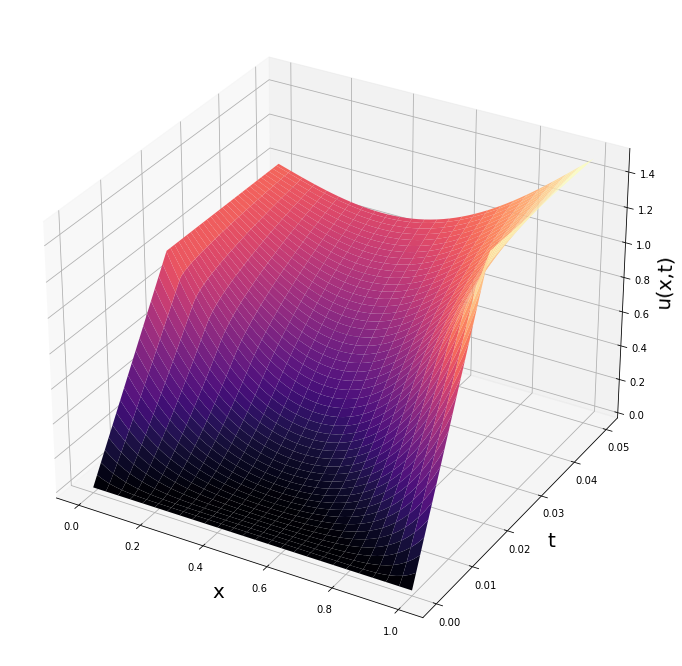
\includegraphics[width=\linewidth]{good.png}
\end{subfigure} %
\begin{subfigure}{.7\linewidth}
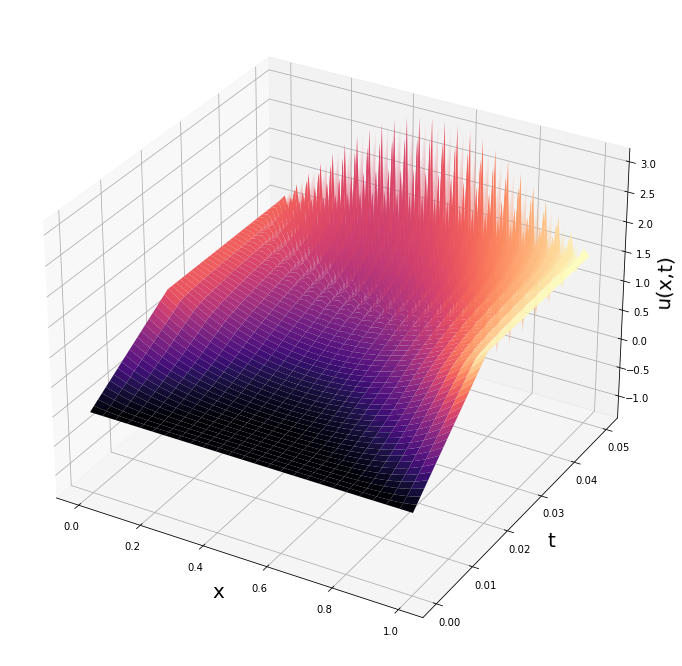
\includegraphics[width=\linewidth]{bad.png}
\end{subfigure}
\caption{Plots of the results of the forward difference method approximation for various timesteps. \textbf{Top:} Approximation with 1000 timesteps. We can see the boundary conditions growing until $t*$, and the heat from the boundaries flowing to raise the temperature in the interior of the bar. \textbf{Bottom:} The same problem solved with 992 timesteps. The solution is well-behaved for small $t$, but we see high frequency noise becoming severe and growing larger at the end of the time interval. }
\end{figure}

\end{document}